\chapter{User manual}
\label{manual}

HTML pages in the~style of common GRASS GIS user manuals were created. In this
chapter, they will be attached. Firstly, they will introduce Mask R-CNN tools
generally and then each module separately.

\section{Mask R-CNN tools}

\subsection*{DESCRIPTION}

Mask R-CNN tools allow the~user to train his own model and use it for
a~detection of objects, or to use a~model provided by someone else. It can be seen 
as a~supervised classification using convolutional neural networks.

The training is done using module \emph{ann.maskrcnn.train}. The~user feeds
the~module with training data consisting of images and masks for each instance of 
intended classes and gets a~model. For difficult tasks and when not using
a~pretrained model, the~training may take even weeks; in case of a~good pretrained 
model and powerful PC with GPU support, the~training could get good results 
after 1 day and even less.

When the~user has a~model, it can be used for the~detection. 
\emph{ann.maskrcnn.detect} detects classes learned during the~training and 
extracts from given images vectors corresponding to detected objects. Objects 
can be extracted either as areas or points. 

\subsection*{DEPENDENCIES}

\emph{ann.maskrcnn.*} modules contain a~lot of external python dependencies.
To run modules, it is necessary to have them installed. Modules use Python 3, so
please install Python 3 versions.

\liststyleLi
\begin{itemize}
\item NumPy
\item Pillow
\item SciPy
\item Cython
\item scikit-image
\item OSGeo
\item TensorFlow
\item Keras
\item h5py
\end{itemize}

After dependencies are fulfilled, modules can be installed using
\emph{g.extension} module:
{\footnotesize
\begin{lstlisting}
g.extension extension=maskrcnn url=path/to/the/maskrcnn/folder
\end{lstlisting}
}


\subsection*{GRASS GIS PATCH}

Unfortunately, python3 is not fully supported by GRASS GIS yet. To use
environment setting flags like \emph{--overwrite}, the~user has to update
his GRASS GIS with the~following patch:

{\footnotesize
\begin{lstlisting}[breaklines=true]
===================================================================
--- lib/python/script/core.py	(revision 72644)
+++ lib/python/script/core.py	(working copy)
@@ -746,7 +746,7 @@
         elif var.startswith(b'opt_'):
             options[var[4:]] = val
         elif var in [b'GRASS_OVERWRITE', b'GRASS_VERBOSE']:
-            os.environ[var] = val
+            os.environ[var.decode("utf-8")] = val.decode("utf-8")
         else:
             raise SyntaxError("invalid output from g.parser: %s" % line)
\end{lstlisting}
}

\subsection*{MODULES}

\emph{ann.maskrcnn.train},\emph{ }\emph{ann.maskrcnn.detect}\emph{ }

\clearpage

\section{ann.maskrcnn.train}

\subsection*{NAME}

\textbf{ann.maskrcnn.train -} Train your Mask R-CNN network.

\subsection*{SYNOPSIS}

\begin{flushleft}
\textbf{ann.maskrcnn.train} 

\textbf{ann.maskrcnn.train -{}-help}

\textbf{ann.maskrcnn.train} [\textbf{-esbn}] \textbf{training\_dataset}=name [\textbf{model}=string] \tab\ \textbf{classes}=string[,string,...] \textbf{logs}=name \textbf{name}=string [\textbf{epochs}=value] \tab\ [\textbf{steps\_per\_epoch}=value] [\textbf{rois\_per\_image}=value] \tab\ [\textbf{images\_per\_gpu}=value] [\textbf{gpu\_count}=value] \tab\ [\textbf{mini\_mask\_size}=value[,value,...]] [\textbf{validation\_steps}=value] \tab\ [\textbf{images\_min\_dim}=value] [\textbf{images\_max\_dim}=value] \tab\ [\textbf{backbone}=string] [\textbf{-{}-overwrite}] [\textbf{-{}-help}] [\textbf{-{}-verbose}] [\textbf{-{}-quiet}] [\textbf{-{}-ui}]
\end{flushleft}

\subsubsection*{Flags:}
\begin{flushleft}
  \textbf{-e}
  
  \tab Pretrained weights were trained on another classes / resolution / sizes
  
  \textbf{-s}
  
  \tab Do not use 10 \% of images and save their list to logs dir
  
  \textbf{-b}
  
  \tab Train also batch normalization layers (not recommended for small batches)

  \textbf{-n}
  
  \tab No resizing or padding of images (images must be of the~same size)
  
  \textbf{-{}-overwrite}
  
  \tab Allow output files to overwrite existing files
  
  \textbf{-{}-help}
  
  \tab Print usage summary
  
  \textbf{-{}-verbose}
  
  \tab Verbose module output
  
  \textbf{-{}-quiet}
  
  \tab Quiet module output
  
  \textbf{-{}-ui}
  
  \tab Force launching GUI dialog
\end{flushleft}

\subsubsection*{Parameters:}

\begin{flushleft}
\textbf{training\_dataset}=name \textbf{[required]}

\tab Path to the~dataset with images and masks

\textbf{model}=string

\tab Path to the~.h5 file to use as initial values

\tab Keep empty to train from a~scratch

\textbf{classes}=string[,string,...] \textbf{[required]}
           
\tab Names of classes separated with ","

\textbf{logs}=name \textbf{[required]}

\tab Path to the~directory in which will be models saved

\textbf{name}=string \textbf{[required]}

\tab Name for output models

\textbf{epochs}=value

\tab Number of epochs

\tab default: 200

\textbf{steps\_per\_epoch}=value

\tab Steps per each epoch

\tab default: 3000

\textbf{rois\_per\_image}=value

\tab How many ROIs train per image

\tab default: 64

\textbf{images\_per\_gpu}=value

\tab Number of images per GPU

\tab Bigger number means faster training but needs a~bigger GPU

\tab default: 1

\textbf{gpu\_count}=value

\tab Number of GPUs to be used

\tab default: 1

\textbf{mini\_mask\_size}=value[,value,...]

\tab Size of mini mask separated with ","

\tab To use full sized masks, keep empty.

\tab Mini mask saves memory at the~expense of precision

\textbf{validation\_steps}=value

\tab Number of validation steps

\tab Bigger number means more accurate estimation of the~model precision

\tab default: 100

\textbf{images\_min\_dim}=value

\tab Minimum length of images sides

\tab Images will be resized to have their shortest side at least of this value

\tab Has to be a~multiple of 64

\tab default: 256

\textbf{images\_max\_dim}=value

\tab Maximum length of images sides

\tab Images will be resized to have their longest side of this value

\tab Has to be a~multiple of 64

\tab default: 1280

\textbf{backbone}=string

\tab Backbone architecture

\tab options: resnet50, resnet101

\tab default: resnet101
\end{flushleft}

\subsection*{DESCRIPTION}
\textstyleEmphasis{ann.maskrcnn.train} allows the user to train a~Mask R-CNN model
on his own dataset. The~dataset has to be prepared in a~predefined structure. 

\subsubsection*{DATASET STRUCTURE}
Training dataset should be in the~following structure: 

\liststyleLi
\begin{itemize}
\item dataset-directory
\begin{itemize}
\item imagenumber 

\begin{itemize}
\item imagenumber.jpg (training image) 
\item imagenumber-class1-number.png (mask for one instance of class1) 
\item imagenumber-class1-number.png (mask for another instance of class1) 
\item ... 
\end{itemize}
\item imagenumber2 

\begin{itemize}
\item imagenumber2.jpg 
\item imagenumber2-class1-number.png (mask for one instance of class1) 
\item imagenumber2-class2-number.png (mask for another class instance) 
\item ... 
\end{itemize}
\end{itemize}
\end{itemize}

The described structure of directories is required. Pictures must be *.jpg files
with 3 channels (for example RGB), masks must be *.png files consisting of
numbers between 1 and 255 (object instance) and 0s (elsewhere). A~mask file for
each instance of an object should be provided separately distinguished by the
suffix number. 

\subsection*{NOTES}
If you are using initial weights (the \textstyleEmphasis{model} parameter),
epochs are divided into three segments. Firstly training layers 5+, then
fine-tuning layers 4+ and the~last segment is fine-tuning the~whole
architecture. Ending number of epochs is shown for your segment, not for the
whole training. 

The usage of the~\textstyleEmphasis{{}-b} flag will result in an activation of
batch normalization layers training. By default, this option is set to False,
as it is not recommended to train them when using just small batches (batch is
defined by the~\textstyleEmphasis{images\_per\_gpu} parameter). 

If the~dataset consists of images of the~same size, the~user may use the
\textstyleEmphasis{{}-n} flag to avoid resizing or padding of images. When the
flag is not used, images are resized to have their longer side equal to the
value of the~\textstyleEmphasis{images\_max\_dim} parameter and the~shorter
side longer or equal to the~value of the~\textstyleEmphasis{images\_min\_dim}
parameter and zero-padded to be of shape \verb|images\_max\_dim| $\times$
\verb|images\_max\_dim|. It results in the~fact that even images of different
sizes may be used. 

After each epoch, the~current model is saved. It allows the~user to stop the~training
when he feels satisfied with loss functions. It also allows the~user to
test models even during the~training (and, again, stop it even before the~last
epoch). 

\subsection*{EXAMPLES}
Dataset for examples: 

\liststyleLii
\begin{itemize}
\item crops 

\begin{itemize}
\item 000000 

\begin{itemize}
\item 000000.jpg 
\item 000000-corn-0.png 
\item 000000-corn-1.png 
\item ... 
\end{itemize}
\item 000001 

\begin{itemize}
\item 000001.jpg 
\item 000001-corn-0.png 
\item 000001-rice-0.png 
\item ... 
\end{itemize}
\end{itemize}
\end{itemize}

\subsubsection*{Training from scratch}

{\footnotesize
\begin{lstlisting}[breaklines=true]
ann.maskrcnn.train training_dataset=/home/user/Documents/crops classes=corn,rice logs=/home/user/Documents/logs name=crops
\end{lstlisting}
}

After default number of epochs, we will get a~model where the~first class is
trained to detect corn fields and the~second one to detect rice fields. 

If we use the~command with reversed classes order, we will get a~model where the
first class is trained to detect rice fields and the~second one to detect corn
fields:

{\footnotesize
\begin{lstlisting}[breaklines=true]
ann.maskrcnn.train training_dataset=/home/user/Documents/crops classes=rice,corn logs=/home/user/Documents/logs name=crops
\end{lstlisting}
}

The name of the~model does not have to be the~same as the~dataset folder but
should be referring to the~task of the~dataset. A~good name for this one
(referring also to the~order of classes) could be also this one: 

{\footnotesize
\begin{lstlisting}[breaklines=true]
ann.maskrcnn.train training_dataset=/home/user/Documents/crops classes=rice,corn logs=/home/user/Documents/logs name=rice_corn
\end{lstlisting}
}

\subsubsection*{Training from a~pretrained model}
We can use a~pretrained model to make our training faster. It is necessary for
the~model to be trained on the~same channels and similar features, but it does
not have to be the~same ones (e.g. model trained on swimming pools in maps can
be used for a~training on buildings in maps). 

A model trained on different classes (use \textstyleEmphasis{{}-e} flag to
exclude head weights):

{\footnotesize
\begin{lstlisting}[breaklines=true]
ann.maskrcnn.train training_dataset=/home/user/Documents/crops classes=corn,rice logs=/home/user/Documents/logs name=crops model=/home/user/Documents/models/buildings.h5 -e
\end{lstlisting}
}

A model trained on the~same classes:

{\footnotesize
\begin{lstlisting}[breaklines=true]
ann.maskrcnn.train training_dataset=/home/user/Documents/crops classes=corn,rice logs=/home/user/Documents/logs name=crops model=/home/user/Documents/models/corn_rice.h5
\end{lstlisting}
}

\subsubsection*{Fine-tuning a~model}
It is also possible to stop your training and then continue. To continue in the
training, just use the~last saved epoch as a~pretrained model:

{\footnotesize
\begin{lstlisting}[breaklines=true]
ann.maskrcnn.train training_dataset=/home/user/Documents/crops classes=corn,rice logs=/home/user/Documents/logs name=crops model=/home/user/Documents/models/mask_rcnn_crops_0005.h5
\end{lstlisting}
}

\clearpage

\section{ann.maskrcnn.detect}

\subsection*{NAME}

\textbf{ann.maskrcnn.detect -} Detect features in images using a~Mask R-CNN model.

\subsection*{SYNOPSIS}

\begin{flushleft}
\textbf{ann.maskrcnn.detect} 

\textbf{ann.maskrcnn.detect -{}-help}

\textbf{ann.maskrcnn.detect} [\textbf{-esbn}] \textbf{images\_directory}=name \tab\ \textbf{images\_format}=string \textbf{model}=string \textbf{classes}=string[,string,...] \tab\ [\textbf{masks\_output}=name] [\textbf{output\_type}=string] [\textbf{-{}-overwrite}] [\textbf{-{}-help}] \tab\ [\textbf{-{}-verbose}] [\textbf{-{}-quiet}] [\textbf{-{}-ui}]
\end{flushleft}

\subsubsection*{Flags:}
\begin{flushleft}
  \textbf{-e}
  
  \tab External georeferencing in the~images folder
  
  \textbf{-{}-overwrite}
  
  \tab Allow output files to overwrite existing files
  
  \textbf{-{}-help}
  
  \tab Print usage summary
  
  \textbf{-{}-verbose}
  
  \tab Verbose module output
  
  \textbf{-{}-quiet}
  
  \tab Quiet module output
  
  \textbf{-{}-ui}
  
  \tab Force launching GUI dialog
\end{flushleft}

\subsubsection*{Parameters:}

\begin{flushleft}
\textbf{band1}=name

\tab Name of raster maps to use for detection as the first band
(divided by ",")

\textbf{band2}=name

\tab Name of raster maps to use for detection as the second band
(divided by ",")

\textbf{band3}=name

\tab Name of raster maps to use for detection as the third band
(divided by ",")

\textbf{images\_directory}=name

\tab Path to a~directory with images to detect

\textbf{images\_format}=string

\tab Format suffix of images

\textbf{model}=string \textbf{[required]}

\tab Path to the~.h5 file containing the~model

\textbf{classes}=string[,string,...] \textbf{[required]}
           
\tab Names of classes separated with ","

\textbf{masks\_output}=name

\tab Directory where masks will be saved

\textbf{output\_type}=string

\tab Type of output

\tab options:area, point

\tab default: area
\end{flushleft}

\subsection*{DESCRIPTION}
\textstyleEmphasis{ann.maskrcnn.detect} allows the user to use a~Mask R-CNN
model to detect features in GRASS GIS raster maps or georeferenced files and extract them either as areas or
points. The~module creates a~separate map for each class. 

\subsection*{NOTES}

The detection may be used for raster maps imported in GRASS GIS or for external
files (or using both). To use raster maps in GRASS GIS, you need to pass them
in three bands following the order used during the training, e.g. if the
training has been made on RGB images, use \textstyleEmphasis{band1=*.red</em},
\textstyleEmphasis{band1=*.green} and \textstyleEmphasis{band3=*.blue}. To
pass multiple images, put more maps into \textstyleEmphasis{band*} parameters,
divided by ",".

The detection may be used also for multiple external files. However, all files
for the detection must be in one directory specified in the
\textstyleEmphasis{images\_directory} parameter. Even when using only one
image, the~module finds it through this parameter. 

When detecting, you can use new names of classes. Classes in the~model are not
referenced by their name, but by their order. It means that if the~model was
trained with classes \textstyleEmphasis{corn,rice} and you use
\textstyleEmphasis{ann.maskrcnn.detect} with classes
\textstyleEmphasis{zea,oryza}, zea areas will present areas detected as corn
and oryza areas will present areas detected as rice. 

If the~external file is georeferenced externally (by a~worldfile or an
\textstyleEmphasis{.aux.xml} file), please use \textstyleEmphasis{{}-e} flag. 

\subsection*{EXAMPLES}
\subsubsection*{Detect buildings and lakes and import them as areas}

One map imported in GRASS GIS:

{\footnotesize
\begin{lstlisting}[breaklines=true]
ann.maskrcnn.detect band1=map1.red band2=map1.green band3=map1.blue classes=buildings,lakes model=/home/user/Documents/logs/mask_rcnn_buildings_lakes_0100.h5
\end{lstlisting}
}

\ \linebreak Two maps (map1, map2) imported in GRASS GIS:

{\footnotesize
\begin{lstlisting}[breaklines=true]
ann.maskrcnn.detect band1=map1.red,map2.red band2=map1.green,map2.green band3=map1.blue,map2.blue classes=buildings,lakes model=/home/user/Documents/logs/mask_rcnn_buildings_lakes_0100.h5
\end{lstlisting}
}

\ \linebreak External files, the~georeferencing is internal (GeoTIFF): 

{\footnotesize
\begin{lstlisting}[breaklines=true]
ann.maskrcnn.detect images_directory=/home/user/Documents/georeferenced_images classes=buildings,lakes model=/home/user/Documents/logs/mask_rcnn_buildings_lakes_0100.h5 images_format=tif
\end{lstlisting}
}

\ \linebreak External files, the~georeferencing is external: 

{\footnotesize
\begin{lstlisting}[breaklines=true]
ann.maskrcnn.detect images_directory=/home/user/Documents/georeferenced_images classes=buildings,lakes model=/home/user/Documents/logs/mask_rcnn_buildings_lakes_0100.h5 images_format=png  -e
\end{lstlisting}
}

\subsubsection*{Detect cottages and plattenbaus and import them as points}

{\footnotesize
\begin{lstlisting}[breaklines=true]
ann.maskrcnn.detect ann.maskrcnn.detect band1=map1.red band2=map1.green band3=map1.blue classes=buildings,lakes model=/home/user/Documents/logs/mask_rcnn_buildings_lakes_0100.h5 output_type=point
\end{lstlisting}
}

\chapter{Examples}
\label{examples}

In the~following chapter, few results obtained during tests of modules will be
presented. Firstly a~module trained to detect football and tennis pitches, then 
a module trained to detect buildings.

\section{Pitches}

The model for detecting football and tennis pitches was trained on a~Debian 
server with 16 CPUs Intel Xeon E5540 (8 CPUs were in the~use) and with memory
49~GBs. The~processor base frequency of Intel Xeon E5540 is 2.53 GHz and the~cache 
is 8~MB. The~training used a~model trained on the~MS COCO dataset as
a~pre-trained model and the~training took one month.

The training dataset consisted of Bing 
maps\footnote{\url{https://www.bing.com/maps}} tiles with zoom level 18 
(resolution 0.6 m per pixel) and masks corresponding to above-mentioned pitches. 
The training dataset consisted of almost 54000 images (plus masks).

When the~training was stopped, the~loss function was about 0.86.

\begin{figure}[H]
   \centering
	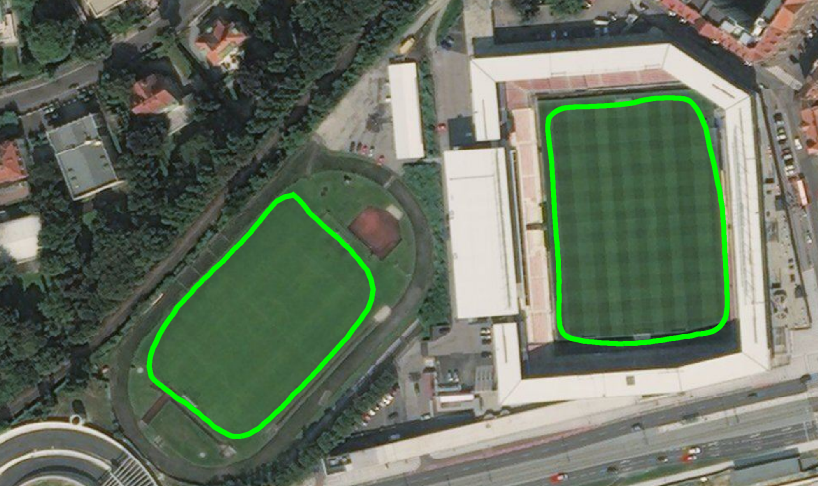
\includegraphics[width=.8\linewidth]{./pictures/out1.png}
	\caption[Detection of football pitches]{An example of the~detection on a~picture containing football pitches}
      \label{fig:football}
\end{figure}

\begin{figure}[H]
   \centering
	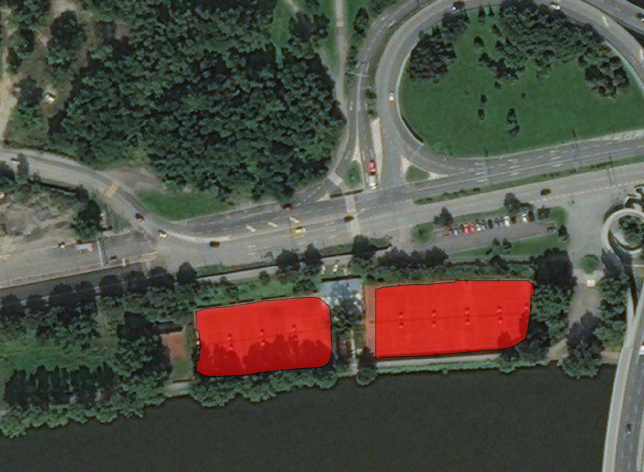
\includegraphics[width=.8\linewidth]{./pictures/out2.png}
	\caption[Detection of tennis pitches]{An example of the~detection on a~picture containing tennis pitches}
      \label{fig:tennis}
\end{figure}

The permission to the usage of Bing map tiles was given to me specifically for 
purposes of this thesis. Unfortunately, the~permission to share the~training 
dataset in e-attachments could not be given to me.


\section{Buildings}

TODO?

\chapter{E-attachments}
\label{attach}

E-attachment of this thesis consists of following features:

\begin{itemize}
	\item The source code of GRASS GIS modules and library
	\item GRASS GIS patch for Python 3
	\item Models mentioned in chapter \ref{examples}
\end{itemize}
